% Created by tikzDevice version 0.12.4 on 2023-07-06 13:18:28
% !TEX encoding = UTF-8 Unicode
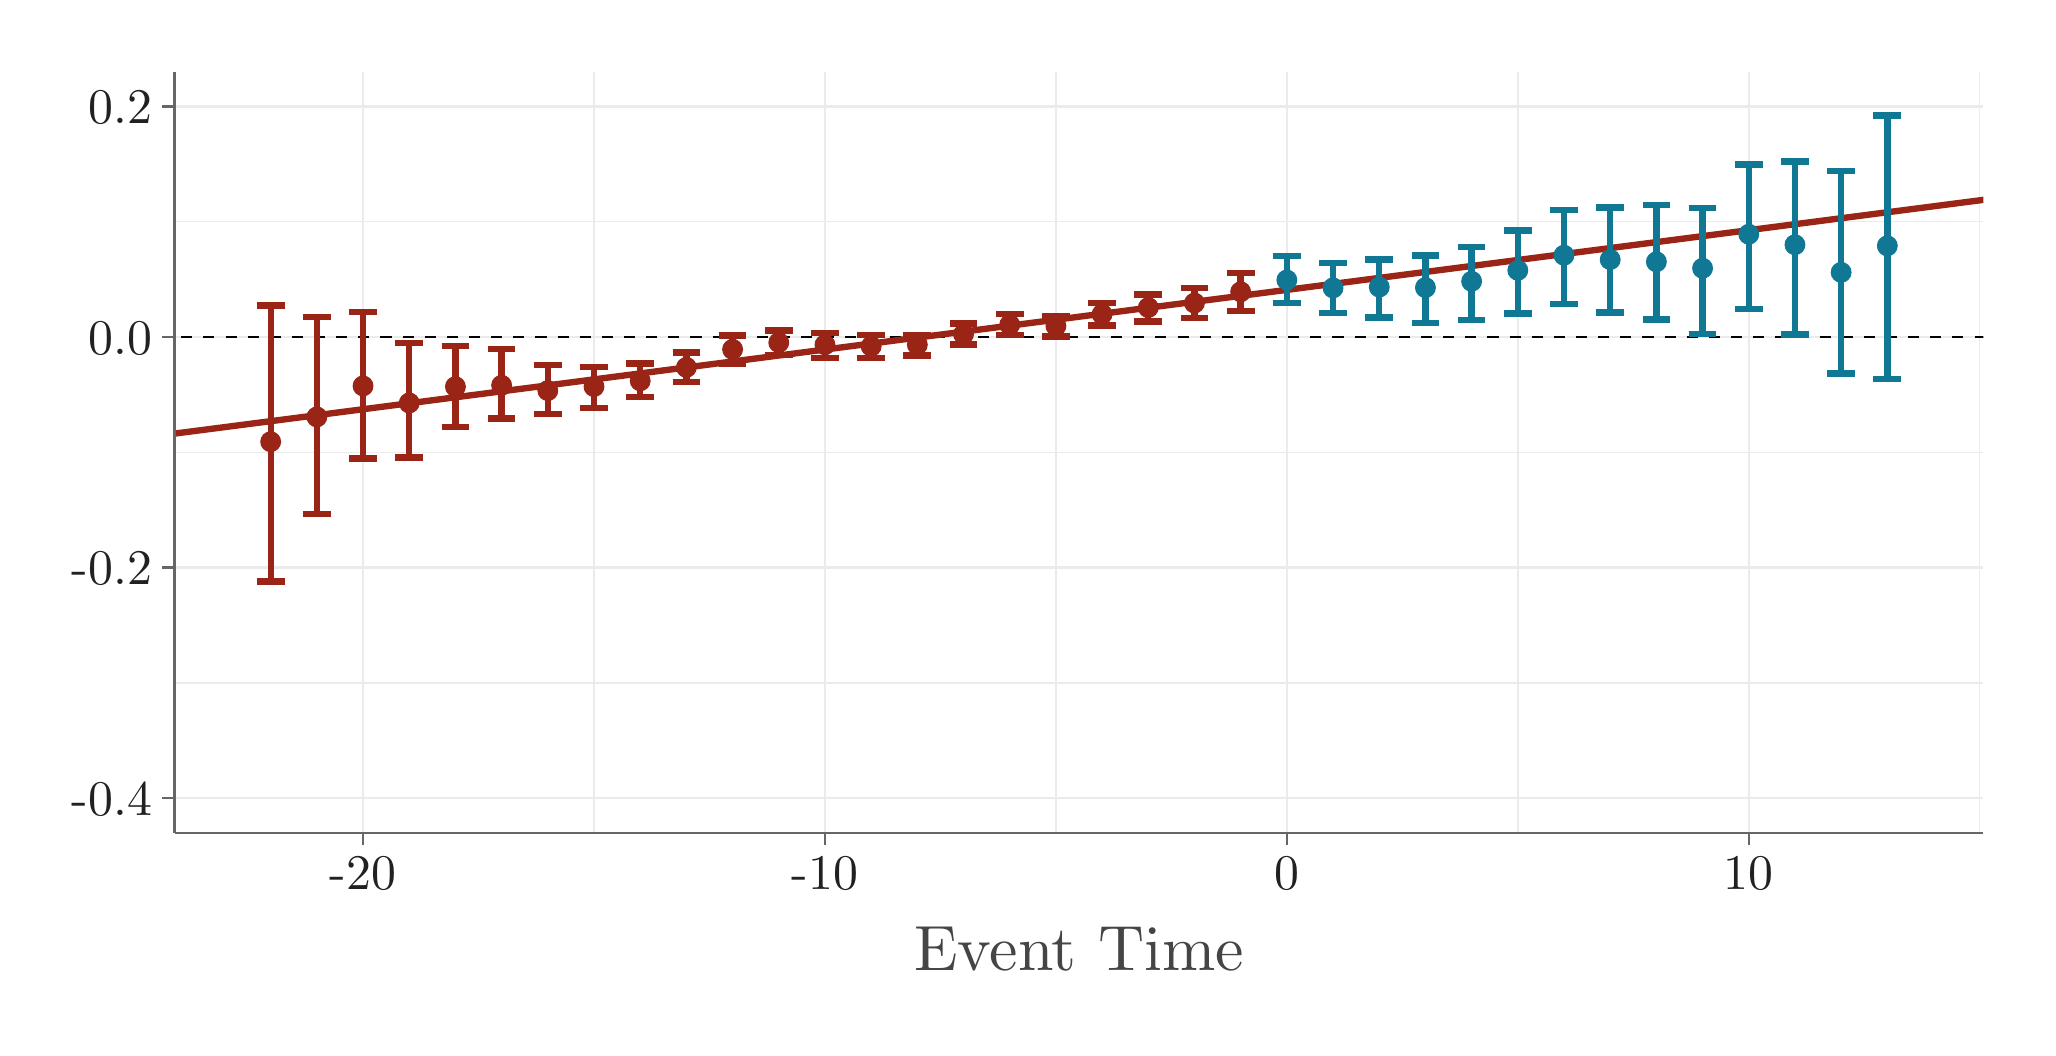
\begin{tikzpicture}[x=1pt,y=1pt]
\definecolor{fillColor}{RGB}{255,255,255}
\path[use as bounding box,fill=fillColor,fill opacity=0.00] (0,0) rectangle (722.70,361.35);
\begin{scope}
\path[clip] (  0.00,  0.00) rectangle (722.70,361.35);
\definecolor{fillColor}{RGB}{255,255,255}

\path[fill=fillColor] (  0.00, -0.00) rectangle (722.70,361.35);
\end{scope}
\begin{scope}
\path[clip] ( 53.09, 70.42) rectangle (706.70,345.35);
\definecolor{fillColor}{RGB}{255,255,255}

\path[fill=fillColor] ( 53.09, 70.42) rectangle (706.70,345.35);
\definecolor{drawColor}{gray}{0.92}

\path[draw=drawColor,line width= 0.5pt,line join=round] ( 53.09,124.58) --
	(706.70,124.58);

\path[draw=drawColor,line width= 0.5pt,line join=round] ( 53.09,207.89) --
	(706.70,207.89);

\path[draw=drawColor,line width= 0.5pt,line join=round] ( 53.09,291.20) --
	(706.70,291.20);

\path[draw=drawColor,line width= 0.5pt,line join=round] (204.64, 70.42) --
	(204.64,345.35);

\path[draw=drawColor,line width= 0.5pt,line join=round] (371.55, 70.42) --
	(371.55,345.35);

\path[draw=drawColor,line width= 0.5pt,line join=round] (538.46, 70.42) --
	(538.46,345.35);

\path[draw=drawColor,line width= 0.5pt,line join=round] (705.36, 70.42) --
	(705.36,345.35);

\path[draw=drawColor,line width= 0.9pt,line join=round] ( 53.09, 82.92) --
	(706.70, 82.92);

\path[draw=drawColor,line width= 0.9pt,line join=round] ( 53.09,166.23) --
	(706.70,166.23);

\path[draw=drawColor,line width= 0.9pt,line join=round] ( 53.09,249.54) --
	(706.70,249.54);

\path[draw=drawColor,line width= 0.9pt,line join=round] ( 53.09,332.85) --
	(706.70,332.85);

\path[draw=drawColor,line width= 0.9pt,line join=round] (121.19, 70.42) --
	(121.19,345.35);

\path[draw=drawColor,line width= 0.9pt,line join=round] (288.10, 70.42) --
	(288.10,345.35);

\path[draw=drawColor,line width= 0.9pt,line join=round] (455.00, 70.42) --
	(455.00,345.35);

\path[draw=drawColor,line width= 0.9pt,line join=round] (621.91, 70.42) --
	(621.91,345.35);
\definecolor{drawColor}{RGB}{0,0,0}

\path[draw=drawColor,line width= 0.9pt,dash pattern=on 4pt off 4pt ,line join=round] (-600.51,249.54) -- (1360.31,249.54);
\definecolor{drawColor}{RGB}{154,36,21}

\path[draw=drawColor,line width= 2.3pt,line join=round] (-600.51,130.21) -- (1360.31,383.59);
\definecolor{fillColor}{RGB}{154,36,21}

\path[draw=drawColor,line width= 0.4pt,line join=round,line cap=round,fill=fillColor] ( 87.81,211.73) circle (  3.57);

\path[draw=drawColor,line width= 0.4pt,line join=round,line cap=round,fill=fillColor] (104.50,220.69) circle (  3.57);

\path[draw=drawColor,line width= 0.4pt,line join=round,line cap=round,fill=fillColor] (121.19,231.88) circle (  3.57);

\path[draw=drawColor,line width= 0.4pt,line join=round,line cap=round,fill=fillColor] (137.88,225.74) circle (  3.57);

\path[draw=drawColor,line width= 0.4pt,line join=round,line cap=round,fill=fillColor] (154.57,231.62) circle (  3.57);

\path[draw=drawColor,line width= 0.4pt,line join=round,line cap=round,fill=fillColor] (171.26,232.12) circle (  3.57);

\path[draw=drawColor,line width= 0.4pt,line join=round,line cap=round,fill=fillColor] (187.95,230.21) circle (  3.57);

\path[draw=drawColor,line width= 0.4pt,line join=round,line cap=round,fill=fillColor] (204.64,231.67) circle (  3.57);

\path[draw=drawColor,line width= 0.4pt,line join=round,line cap=round,fill=fillColor] (221.34,233.73) circle (  3.57);

\path[draw=drawColor,line width= 0.4pt,line join=round,line cap=round,fill=fillColor] (238.03,238.59) circle (  3.57);

\path[draw=drawColor,line width= 0.4pt,line join=round,line cap=round,fill=fillColor] (254.72,245.11) circle (  3.57);

\path[draw=drawColor,line width= 0.4pt,line join=round,line cap=round,fill=fillColor] (271.41,247.56) circle (  3.57);

\path[draw=drawColor,line width= 0.4pt,line join=round,line cap=round,fill=fillColor] (288.10,246.76) circle (  3.57);

\path[draw=drawColor,line width= 0.4pt,line join=round,line cap=round,fill=fillColor] (304.79,246.22) circle (  3.57);

\path[draw=drawColor,line width= 0.4pt,line join=round,line cap=round,fill=fillColor] (321.48,246.77) circle (  3.57);

\path[draw=drawColor,line width= 0.4pt,line join=round,line cap=round,fill=fillColor] (338.17,250.55) circle (  3.57);

\path[draw=drawColor,line width= 0.4pt,line join=round,line cap=round,fill=fillColor] (354.86,254.00) circle (  3.57);

\path[draw=drawColor,line width= 0.4pt,line join=round,line cap=round,fill=fillColor] (371.55,253.55) circle (  3.57);

\path[draw=drawColor,line width= 0.4pt,line join=round,line cap=round,fill=fillColor] (388.24,257.81) circle (  3.57);

\path[draw=drawColor,line width= 0.4pt,line join=round,line cap=round,fill=fillColor] (404.93,260.21) circle (  3.57);

\path[draw=drawColor,line width= 0.4pt,line join=round,line cap=round,fill=fillColor] (421.62,261.84) circle (  3.57);

\path[draw=drawColor,line width= 0.4pt,line join=round,line cap=round,fill=fillColor] (438.31,265.89) circle (  3.57);
\definecolor{drawColor}{RGB}{16,120,149}
\definecolor{fillColor}{RGB}{16,120,149}

\path[draw=drawColor,line width= 0.4pt,line join=round,line cap=round,fill=fillColor] (455.00,270.17) circle (  3.57);

\path[draw=drawColor,line width= 0.4pt,line join=round,line cap=round,fill=fillColor] (471.70,267.31) circle (  3.57);

\path[draw=drawColor,line width= 0.4pt,line join=round,line cap=round,fill=fillColor] (488.39,267.62) circle (  3.57);

\path[draw=drawColor,line width= 0.4pt,line join=round,line cap=round,fill=fillColor] (505.08,267.42) circle (  3.57);

\path[draw=drawColor,line width= 0.4pt,line join=round,line cap=round,fill=fillColor] (521.77,269.70) circle (  3.57);

\path[draw=drawColor,line width= 0.4pt,line join=round,line cap=round,fill=fillColor] (538.46,273.67) circle (  3.57);

\path[draw=drawColor,line width= 0.4pt,line join=round,line cap=round,fill=fillColor] (555.15,279.13) circle (  3.57);

\path[draw=drawColor,line width= 0.4pt,line join=round,line cap=round,fill=fillColor] (571.84,277.54) circle (  3.57);

\path[draw=drawColor,line width= 0.4pt,line join=round,line cap=round,fill=fillColor] (588.53,276.74) circle (  3.57);

\path[draw=drawColor,line width= 0.4pt,line join=round,line cap=round,fill=fillColor] (605.22,274.42) circle (  3.57);

\path[draw=drawColor,line width= 0.4pt,line join=round,line cap=round,fill=fillColor] (621.91,286.70) circle (  3.57);

\path[draw=drawColor,line width= 0.4pt,line join=round,line cap=round,fill=fillColor] (638.60,282.91) circle (  3.57);

\path[draw=drawColor,line width= 0.4pt,line join=round,line cap=round,fill=fillColor] (655.29,272.93) circle (  3.57);

\path[draw=drawColor,line width= 0.4pt,line join=round,line cap=round,fill=fillColor] (671.98,282.51) circle (  3.57);
\definecolor{drawColor}{RGB}{154,36,21}

\path[draw=drawColor,line width= 2.3pt,line join=round] ( 82.80,261.00) --
	( 92.82,261.00);

\path[draw=drawColor,line width= 2.3pt,line join=round] ( 87.81,261.00) --
	( 87.81,161.22);

\path[draw=drawColor,line width= 2.3pt,line join=round] ( 82.80,161.22) --
	( 92.82,161.22);

\path[draw=drawColor,line width= 2.3pt,line join=round] ( 99.49,256.75) --
	(109.51,256.75);

\path[draw=drawColor,line width= 2.3pt,line join=round] (104.50,256.75) --
	(104.50,185.57);

\path[draw=drawColor,line width= 2.3pt,line join=round] ( 99.49,185.57) --
	(109.51,185.57);

\path[draw=drawColor,line width= 2.3pt,line join=round] (116.18,258.55) --
	(126.20,258.55);

\path[draw=drawColor,line width= 2.3pt,line join=round] (121.19,258.55) --
	(121.19,205.63);

\path[draw=drawColor,line width= 2.3pt,line join=round] (116.18,205.63) --
	(126.20,205.63);

\path[draw=drawColor,line width= 2.3pt,line join=round] (132.87,247.47) --
	(142.89,247.47);

\path[draw=drawColor,line width= 2.3pt,line join=round] (137.88,247.47) --
	(137.88,206.09);

\path[draw=drawColor,line width= 2.3pt,line join=round] (132.87,206.09) --
	(142.89,206.09);

\path[draw=drawColor,line width= 2.3pt,line join=round] (149.57,246.42) --
	(159.58,246.42);

\path[draw=drawColor,line width= 2.3pt,line join=round] (154.57,246.42) --
	(154.57,216.94);

\path[draw=drawColor,line width= 2.3pt,line join=round] (149.57,216.94) --
	(159.58,216.94);

\path[draw=drawColor,line width= 2.3pt,line join=round] (166.26,245.21) --
	(176.27,245.21);

\path[draw=drawColor,line width= 2.3pt,line join=round] (171.26,245.21) --
	(171.26,220.07);

\path[draw=drawColor,line width= 2.3pt,line join=round] (166.26,220.07) --
	(176.27,220.07);

\path[draw=drawColor,line width= 2.3pt,line join=round] (182.95,239.34) --
	(192.96,239.34);

\path[draw=drawColor,line width= 2.3pt,line join=round] (187.95,239.34) --
	(187.95,221.86);

\path[draw=drawColor,line width= 2.3pt,line join=round] (182.95,221.86) --
	(192.96,221.86);

\path[draw=drawColor,line width= 2.3pt,line join=round] (199.64,238.70) --
	(209.65,238.70);

\path[draw=drawColor,line width= 2.3pt,line join=round] (204.64,238.70) --
	(204.64,223.84);

\path[draw=drawColor,line width= 2.3pt,line join=round] (199.64,223.84) --
	(209.65,223.84);

\path[draw=drawColor,line width= 2.3pt,line join=round] (216.33,240.01) --
	(226.34,240.01);

\path[draw=drawColor,line width= 2.3pt,line join=round] (221.34,240.01) --
	(221.34,227.95);

\path[draw=drawColor,line width= 2.3pt,line join=round] (216.33,227.95) --
	(226.34,227.95);

\path[draw=drawColor,line width= 2.3pt,line join=round] (233.02,244.02) --
	(243.03,244.02);

\path[draw=drawColor,line width= 2.3pt,line join=round] (238.03,244.02) --
	(238.03,233.41);

\path[draw=drawColor,line width= 2.3pt,line join=round] (233.02,233.41) --
	(243.03,233.41);

\path[draw=drawColor,line width= 2.3pt,line join=round] (249.71,250.13) --
	(259.72,250.13);

\path[draw=drawColor,line width= 2.3pt,line join=round] (254.72,250.13) --
	(254.72,239.89);

\path[draw=drawColor,line width= 2.3pt,line join=round] (249.71,239.89) --
	(259.72,239.89);

\path[draw=drawColor,line width= 2.3pt,line join=round] (266.40,251.89) --
	(276.41,251.89);

\path[draw=drawColor,line width= 2.3pt,line join=round] (271.41,251.89) --
	(271.41,242.99);

\path[draw=drawColor,line width= 2.3pt,line join=round] (266.40,242.99) --
	(276.41,242.99);

\path[draw=drawColor,line width= 2.3pt,line join=round] (283.09,251.11) --
	(293.10,251.11);

\path[draw=drawColor,line width= 2.3pt,line join=round] (288.10,251.11) --
	(288.10,242.04);

\path[draw=drawColor,line width= 2.3pt,line join=round] (283.09,242.04) --
	(293.10,242.04);

\path[draw=drawColor,line width= 2.3pt,line join=round] (299.78,250.21) --
	(309.80,250.21);

\path[draw=drawColor,line width= 2.3pt,line join=round] (304.79,250.21) --
	(304.79,242.04);

\path[draw=drawColor,line width= 2.3pt,line join=round] (299.78,242.04) --
	(309.80,242.04);

\path[draw=drawColor,line width= 2.3pt,line join=round] (316.47,250.30) --
	(326.49,250.30);

\path[draw=drawColor,line width= 2.3pt,line join=round] (321.48,250.30) --
	(321.48,242.86);

\path[draw=drawColor,line width= 2.3pt,line join=round] (316.47,242.86) --
	(326.49,242.86);

\path[draw=drawColor,line width= 2.3pt,line join=round] (333.16,254.49) --
	(343.18,254.49);

\path[draw=drawColor,line width= 2.3pt,line join=round] (338.17,254.49) --
	(338.17,246.89);

\path[draw=drawColor,line width= 2.3pt,line join=round] (333.16,246.89) --
	(343.18,246.89);

\path[draw=drawColor,line width= 2.3pt,line join=round] (349.85,257.86) --
	(359.87,257.86);

\path[draw=drawColor,line width= 2.3pt,line join=round] (354.86,257.86) --
	(354.86,250.29);

\path[draw=drawColor,line width= 2.3pt,line join=round] (349.85,250.29) --
	(359.87,250.29);

\path[draw=drawColor,line width= 2.3pt,line join=round] (366.54,257.27) --
	(376.56,257.27);

\path[draw=drawColor,line width= 2.3pt,line join=round] (371.55,257.27) --
	(371.55,249.78);

\path[draw=drawColor,line width= 2.3pt,line join=round] (366.54,249.78) --
	(376.56,249.78);

\path[draw=drawColor,line width= 2.3pt,line join=round] (383.23,261.80) --
	(393.25,261.80);

\path[draw=drawColor,line width= 2.3pt,line join=round] (388.24,261.80) --
	(388.24,253.75);

\path[draw=drawColor,line width= 2.3pt,line join=round] (383.23,253.75) --
	(393.25,253.75);

\path[draw=drawColor,line width= 2.3pt,line join=round] (399.93,264.92) --
	(409.94,264.92);

\path[draw=drawColor,line width= 2.3pt,line join=round] (404.93,264.92) --
	(404.93,255.22);

\path[draw=drawColor,line width= 2.3pt,line join=round] (399.93,255.22) --
	(409.94,255.22);

\path[draw=drawColor,line width= 2.3pt,line join=round] (416.62,267.29) --
	(426.63,267.29);

\path[draw=drawColor,line width= 2.3pt,line join=round] (421.62,267.29) --
	(421.62,256.43);

\path[draw=drawColor,line width= 2.3pt,line join=round] (416.62,256.43) --
	(426.63,256.43);

\path[draw=drawColor,line width= 2.3pt,line join=round] (433.31,272.79) --
	(443.32,272.79);

\path[draw=drawColor,line width= 2.3pt,line join=round] (438.31,272.79) --
	(438.31,258.95);

\path[draw=drawColor,line width= 2.3pt,line join=round] (433.31,258.95) --
	(443.32,258.95);
\definecolor{drawColor}{RGB}{16,120,149}

\path[draw=drawColor,line width= 2.3pt,line join=round] (450.00,278.88) --
	(460.01,278.88);

\path[draw=drawColor,line width= 2.3pt,line join=round] (455.00,278.88) --
	(455.00,261.95);

\path[draw=drawColor,line width= 2.3pt,line join=round] (450.00,261.95) --
	(460.01,261.95);

\path[draw=drawColor,line width= 2.3pt,line join=round] (466.69,276.42) --
	(476.70,276.42);

\path[draw=drawColor,line width= 2.3pt,line join=round] (471.70,276.42) --
	(471.70,258.23);

\path[draw=drawColor,line width= 2.3pt,line join=round] (466.69,258.23) --
	(476.70,258.23);

\path[draw=drawColor,line width= 2.3pt,line join=round] (483.38,277.57) --
	(493.39,277.57);

\path[draw=drawColor,line width= 2.3pt,line join=round] (488.39,277.57) --
	(488.39,256.66);

\path[draw=drawColor,line width= 2.3pt,line join=round] (483.38,256.66) --
	(493.39,256.66);

\path[draw=drawColor,line width= 2.3pt,line join=round] (500.07,279.07) --
	(510.08,279.07);

\path[draw=drawColor,line width= 2.3pt,line join=round] (505.08,279.07) --
	(505.08,254.67);

\path[draw=drawColor,line width= 2.3pt,line join=round] (500.07,254.67) --
	(510.08,254.67);

\path[draw=drawColor,line width= 2.3pt,line join=round] (516.76,282.15) --
	(526.77,282.15);

\path[draw=drawColor,line width= 2.3pt,line join=round] (521.77,282.15) --
	(521.77,255.80);

\path[draw=drawColor,line width= 2.3pt,line join=round] (516.76,255.80) --
	(526.77,255.80);

\path[draw=drawColor,line width= 2.3pt,line join=round] (533.45,288.00) --
	(543.47,288.00);

\path[draw=drawColor,line width= 2.3pt,line join=round] (538.46,288.00) --
	(538.46,258.00);

\path[draw=drawColor,line width= 2.3pt,line join=round] (533.45,258.00) --
	(543.47,258.00);

\path[draw=drawColor,line width= 2.3pt,line join=round] (550.14,295.44) --
	(560.16,295.44);

\path[draw=drawColor,line width= 2.3pt,line join=round] (555.15,295.44) --
	(555.15,261.49);

\path[draw=drawColor,line width= 2.3pt,line join=round] (550.14,261.49) --
	(560.16,261.49);

\path[draw=drawColor,line width= 2.3pt,line join=round] (566.83,296.32) --
	(576.85,296.32);

\path[draw=drawColor,line width= 2.3pt,line join=round] (571.84,296.32) --
	(571.84,258.38);

\path[draw=drawColor,line width= 2.3pt,line join=round] (566.83,258.38) --
	(576.85,258.38);

\path[draw=drawColor,line width= 2.3pt,line join=round] (583.52,297.26) --
	(593.54,297.26);

\path[draw=drawColor,line width= 2.3pt,line join=round] (588.53,297.26) --
	(588.53,255.92);

\path[draw=drawColor,line width= 2.3pt,line join=round] (583.52,255.92) --
	(593.54,255.92);

\path[draw=drawColor,line width= 2.3pt,line join=round] (600.21,296.19) --
	(610.23,296.19);

\path[draw=drawColor,line width= 2.3pt,line join=round] (605.22,296.19) --
	(605.22,250.59);

\path[draw=drawColor,line width= 2.3pt,line join=round] (600.21,250.59) --
	(610.23,250.59);

\path[draw=drawColor,line width= 2.3pt,line join=round] (616.90,311.84) --
	(626.92,311.84);

\path[draw=drawColor,line width= 2.3pt,line join=round] (621.91,311.84) --
	(621.91,259.73);

\path[draw=drawColor,line width= 2.3pt,line join=round] (616.90,259.73) --
	(626.92,259.73);

\path[draw=drawColor,line width= 2.3pt,line join=round] (633.59,312.95) --
	(643.61,312.95);

\path[draw=drawColor,line width= 2.3pt,line join=round] (638.60,312.95) --
	(638.60,250.51);

\path[draw=drawColor,line width= 2.3pt,line join=round] (633.59,250.51) --
	(643.61,250.51);

\path[draw=drawColor,line width= 2.3pt,line join=round] (650.29,309.64) --
	(660.30,309.64);

\path[draw=drawColor,line width= 2.3pt,line join=round] (655.29,309.64) --
	(655.29,236.43);

\path[draw=drawColor,line width= 2.3pt,line join=round] (650.29,236.43) --
	(660.30,236.43);

\path[draw=drawColor,line width= 2.3pt,line join=round] (666.98,329.59) --
	(676.99,329.59);

\path[draw=drawColor,line width= 2.3pt,line join=round] (671.98,329.59) --
	(671.98,234.47);

\path[draw=drawColor,line width= 2.3pt,line join=round] (666.98,234.47) --
	(676.99,234.47);

\path[] ( 53.09, 70.42) rectangle (706.70,345.35);
\end{scope}
\begin{scope}
\path[clip] (  0.00,  0.00) rectangle (722.70,361.35);
\definecolor{drawColor}{gray}{0.40}

\path[draw=drawColor,line width= 0.9pt,line join=round] ( 53.09, 70.42) --
	( 53.09,345.35);
\end{scope}
\begin{scope}
\path[clip] (  0.00,  0.00) rectangle (722.70,361.35);
\definecolor{drawColor}{gray}{0.13}

\node[text=drawColor,anchor=base east,inner sep=0pt, outer sep=0pt, scale=  1.80] at ( 44.99, 76.72) {-0.4};

\node[text=drawColor,anchor=base east,inner sep=0pt, outer sep=0pt, scale=  1.80] at ( 44.99,160.03) {-0.2};

\node[text=drawColor,anchor=base east,inner sep=0pt, outer sep=0pt, scale=  1.80] at ( 44.99,243.34) {0.0};

\node[text=drawColor,anchor=base east,inner sep=0pt, outer sep=0pt, scale=  1.80] at ( 44.99,326.65) {0.2};
\end{scope}
\begin{scope}
\path[clip] (  0.00,  0.00) rectangle (722.70,361.35);
\definecolor{drawColor}{gray}{0.40}

\path[draw=drawColor,line width= 0.9pt,line join=round] ( 48.59, 82.92) --
	( 53.09, 82.92);

\path[draw=drawColor,line width= 0.9pt,line join=round] ( 48.59,166.23) --
	( 53.09,166.23);

\path[draw=drawColor,line width= 0.9pt,line join=round] ( 48.59,249.54) --
	( 53.09,249.54);

\path[draw=drawColor,line width= 0.9pt,line join=round] ( 48.59,332.85) --
	( 53.09,332.85);
\end{scope}
\begin{scope}
\path[clip] (  0.00,  0.00) rectangle (722.70,361.35);
\definecolor{drawColor}{gray}{0.40}

\path[draw=drawColor,line width= 0.9pt,line join=round] ( 53.09, 70.42) --
	(706.70, 70.42);
\end{scope}
\begin{scope}
\path[clip] (  0.00,  0.00) rectangle (722.70,361.35);
\definecolor{drawColor}{gray}{0.40}

\path[draw=drawColor,line width= 0.9pt,line join=round] (121.19, 65.92) --
	(121.19, 70.42);

\path[draw=drawColor,line width= 0.9pt,line join=round] (288.10, 65.92) --
	(288.10, 70.42);

\path[draw=drawColor,line width= 0.9pt,line join=round] (455.00, 65.92) --
	(455.00, 70.42);

\path[draw=drawColor,line width= 0.9pt,line join=round] (621.91, 65.92) --
	(621.91, 70.42);
\end{scope}
\begin{scope}
\path[clip] (  0.00,  0.00) rectangle (722.70,361.35);
\definecolor{drawColor}{gray}{0.13}

\node[text=drawColor,anchor=base,inner sep=0pt, outer sep=0pt, scale=  1.80] at (121.19, 49.93) {-20};

\node[text=drawColor,anchor=base,inner sep=0pt, outer sep=0pt, scale=  1.80] at (288.10, 49.93) {-10};

\node[text=drawColor,anchor=base,inner sep=0pt, outer sep=0pt, scale=  1.80] at (455.00, 49.93) {0};

\node[text=drawColor,anchor=base,inner sep=0pt, outer sep=0pt, scale=  1.80] at (621.91, 49.93) {10};
\end{scope}
\begin{scope}
\path[clip] (  0.00,  0.00) rectangle (722.70,361.35);
\definecolor{drawColor}{gray}{0.27}

\node[text=drawColor,anchor=base,inner sep=0pt, outer sep=0pt, scale=  2.31] at (379.90, 20.50) {Event Time};
\end{scope}
\end{tikzpicture}
